\chapter{Study Evaluation}
\label{chapter:study_evaluation}
\section{Study Evaluation}
\label{sec:study_evaluation}
The study presented in the last chapter is evaluated with the help of a pre-pilot study and a pilot study. The pre-pilot study was conducted with one participant and focussed on flaws in the process. Subsequently, a pilot study was cibducted with three participants. The pilot study focuss lies on the review of the \exgo\ and the assessment of data. This section describes the findings of the pilot studies and provides improvements for the actual study.

\subsection{Process}
In the beginning, the participant receives a welcome letter. Two participants stated that the information in the welcome letter about how VR headsets work is not necessary. The welcome letter was then shortened by the removal of that passage. The informed consent is signed. The following demographic questionnaire allows putting the study's data into context. During the review of the produced study data, no further questions occurred. The demographic questionnaire needs no further improvements. While the participant reads the welcome letter, the system is set up. The pilot study showed that the time to set up the system and fill in the questionnaires are corresponding.\\
Afterwards, the participant is told that he/she will be equipped with the trackers and where the trackers will be attached. Afterwards, the trackers are attached to the participant. To respect the privacy of the participant, the trackers are handed to the participant and instructions are given on how to attach them. The pilot study showed that the participants had problems following the instructions correctly. For the actual study, the participants will be asked if it is ok that the trackers are attached with the physical help of the study conductor.\\
Next, the participants received information about what to expect in the VR. The instructions contained information about the GV ("You will see one/multiple teachers.") and the task ("Please follow the instructions of the teachers as exactly as possible."). Furthermore, the participant was asked to pay attention to the ergonomics of the movements. Explanations about the speed-mechanic were provided, too ("The teacher will wait for you if you are too far away from the teacher. If that is happening, correct the placements of your feet, and it will go on."). No participant had difficulties understanding the instructions. Additionally, the participant was handed the box to get used to it before seeing its digital pendant in VR. Finally, the calibration of the system was explained ("Please look into the mirror you will see there (study conductor pointing) and extend your arms like this (study conductor performing the T-pose)"). All participants understood how to calibrate easily. The introduction of the mirror as calibration facilitator proved to be helpful and suitable.\\
Subsequently, the camera recordings were started and the participant performed the first task. In this phase of the study, two errors occurred which needed adjustments to the process. In one case, the wrong task was chosen, which made participant 1 (PT1) perform task 1 (T1) two times in different perspectives. PT1 recognised that, too. Before starting the task, an "is everything ok" checklist should be gone through. The second error regards the identification and synchronisation of the video recordings. At the ceiling, a GoPro films the scene from above. A second camera catches the scene from the side of the tracking volume. For identification, a sign held into the view of both cameras. This was forgotten twice. As an improvement, the sign should be placed beforehand in the area both cameras cover.\\
After the participant performed the first task, the participant took off the HMD and is asked to fill in the after-session questionnaire. The trackers stayed at the body of the participant. The pilot study showed that the tracker did not hinder the participants from sitting down and filling in the questionnaire. In the pilot study, a three-minute pause was conducted to allow the participant to recover. During that pause, the participant was asked about his/her wellbeing to check for VR induced motion sickness. All participants stated that they do not need a pause. The demographic questionnaire revealed that all participants were experienced with VR-system and they are used to wear VR HMDs. The pause will be maintained, because a person with no prior exposition to VR could feel different.\\
Session two and three are conducted in the same way as session one. With all three sessions done, the trackers are removed, and the semi-structured interview was conducted. Because the pilot participants were not paid, the pilot study ended here. The planned duration of the study was 75 minutes. All pilot studies took no longer than 55 minutes.  With an additional buffer, the planned study duration can be decreased by 10 minutes to 65 minutes.\\
Additionally, for the study's evaluation, the participants were interviewed to get insights about the studie's and system's flaws. The participants were asked if the explanations were sufficient and if there were any confusing elements or unclear questions in the questionnaires or documents. Finally, the participants' opinion about possible improvements of \exgo\ and the study were asked. The results of those interviews informed section~\ref{sec:studyStructure}, too.\\
To conclude, vast parts of the planned study process proved to be suitable. Adjustments are made to the welcome letter, the trackers' attachment with the study conductor's help, an additional checklist to check the session task and perspective is introduced, and the camera recording identification is improved by placing the sign into the recording area beforehand.

\subsection{\exgo}
All hardware artefacts of \exgo\ are suitable without objections. The study participants rated the box's size and weight as "okay" while still perceiving it as a "physical load". The table's size is sufficient for all three tasks. At no time, the were the participants in danger to collide with a physical artefact. The size of the scale is also sufficient. The box was always placed on the scale safely. The positions and itinerary between mirror, table and scale are without complaint. Regarding the hardware part of \exgo, the pilot study revealed two insights, one related to the trackers and one related to the HMD. The tracker at the hip is attached with a strap around the hip of the participant. While the sub-tasks \textit{lift} and \textit{lower}, the tracker is shifted upwards. The upwards shift affects the avatar's presentation and influences the accuracy measurements hip distance and the RM squat distance and upright stance. To prevent this, the student was asked to wear a belt. The tracker belt was then fixated to the participant belt with a band of velcro. This includes touching the participants in the lower hip area from behind. To prevent participants from feeling uncomfortable during the whole study, the fixation of the two belts should be performed with a clip that the participant can attach themselves. The second insight regarding the hardware of \exgo\ is the cable of the HMD. During the study, the study conductor handled the cable not to influence the participant. In one case, the cable was plugged out during a session. \exgo\ is designed for that case, and plugging in the cable again allows to continue with the session. However, in the actual study, this incident would lead to unusable data for all three sessions of that participant because, meanwhile the cable is plugged in again, the GV will move forward, and the error will be high during this phase. The actual study will benefit from a wireless HMD.\\
One participant stated that he/she could not identify the ownership of the box right away. As soon as the own box is in the participant's hands, it is no problem to tell which is the GV's box and which is the learner's box. However, if both boxes are stationary, the participant could not detect which is the own box. The box should be changed to light transparency for a better distinction between the learner's box and the GV's box. This will also have an influence on the perception of the box during \textit{lift}. During \textit{lift}, the learner's box is occluded by the GV's box for a short time. For conformity, the avatar, table and scale of the GV's should also be rendered with a light transparency.\\
The pilot study served as the last test before the actual study. An essential part of the pilot study is the review of the produced data. During the development, the measures could only be tested individually. The pilot study allowed for the first time to get a whole image. Fortunately, most of the logged data worked as intended. Only minor errors were detected. For spine bend, a last-minute edit caused an incorrect calculation. For EXO, in combination with task 2, an invisible error was detected: the props animation controller, which animates the GV's box, played the wrong task for the ego-centric GV. In EXO, the ego-centric GV is invisible but used to calculate the measurements. For EGO, the learner's avatar identification name (used for looking at, identifying what the learner is visually focussing on) is incorrect. Lastly, Unity3D natively uses comma as decimal separator. Most statistics programs natively use points as decimal separator. A log file of one session contains around 2.5 Million decimal separators. Converting a log file is time-consuming, and therefore, the logging should be changed to use a point as decimal separator.

das zeug aus den questionaires
\subsection{Qualitative Data Aquisition}
After each session, the participant fills in the after-session questionnaire. The last question of the questionnaire is not handed to the participant but asked as interview questions. The feedback of the pilot study's participant was positive, and the three questions were clear and understandable. However, during the analysis of the quantitative data, questions appeared that are worth to ask the study participants:
\begin{itemize}
	\item[Q:] How ergonomic do you think your movements have been?
	\item[A:] Likert scale from 1 (very good) - 7 (very poor)
	\item[] Linked research questions: \todo{todo}
	\item[] The self-assessment of the study participants' performance regarding the ergonomics of the movements can give insights into the participants' feelings. It is expected that the VPs with exo-centiric GVs is rated higher because the posture of the GV can be observed from the side. For example, the back of the GV's bend angle is hard to see in the ego-centric VP. Furthermore, the self-assessment can be put into relation to the quantitative data and used for triangulation.
	\item[Q:] On what did you focus most?
	\item[A:] Two choices: box, teacher
	\item[] Linked research questions: \todo{todo}
	\item[] The assessment of the subjective participants' focus can give insights about the importance of box and avatar for the participants. Presumably, a participant who rates the box over the avatar focussed mainly on the box's accuracy and vice versa. This subjective data can be put into relation to the quantitative data for triangulation. If the quantitative data complies with the qualitative data, the evaluation of the risk metrics can be split into two groups: those who focussed mainly on the box and those who focussed mainly on the avatar. It could be interesting if these two groups score differently regarding the risk metrics.
	\item[Q:] Could you see a teacher at any point in time?
	\item[A:] Two choices: yes, no
	\item[] Linked research questions: none, evaluation of the positions of the GVs
	\item[] The positions of the GVs could only be tested sparsely. This question aims to evaluate if the positions of the GVs were suitable. If the participant crosses "no" during the last interview question this can be addressed in the next question.
\end{itemize}
After all three sessions, the participant is a semi-structured interview. The guideline for the semi-structured interview proved to be suitable. However, during the interviews, one participant could not give a clear prioritisation of which perspective he/she would use if he/she had the choice. I gave in and did not insist on the prioritisation. This caused an inconsistency which becomes clear during the analysis of the qualitative data. In the study, every participant should provide a prioritisation.


\subsection{Acclimatisation Phase}
The first session of each study is the acclimatisation phase, where the learner gets used to \exgo. It is assumed that the learning effect between session one and two is high, and between two and three, nearly no learning effect occurs. To evaluate if this assumption holds, the task completion time (TCT) could give insights because of the \textit{speed mechanic}. The \textit{speed mechanic} regulates the GV animation speed based on the distance between learner and GV and is applied in all perspectives. The higher the learner-GV distance, the lower the speed. A learner who is often located near to the ideal point yields a lower TCT. A formative test in which one participant does the same task in all condition would lead to insights about the learning effect. Such a test was not possible because of the COVID-19 pandemic. Nevertheless, comparing the TCT in the pilot test could at least indicate if the learning effect between session two and three is low by showing similar TCT.\\
Figure~\ref{fig:tct} shows the amount of ms the participants needed more to complete the task compared with the task norm duration (over task norm duration (OTND)). The task norm time is the amount of ms the task needs to complete without the speed-mechanic. The order of the sessions is from left to right. Participant 1 (PT1) had a nearly equal OTND for all three tasks. Because of a mistake in choosing the pilot study task, PT1 faced T1 two times. However, in session three, the OTNT is slightly higher. PT2 shows the expected behaviour, having a high OTND in the first session and a nearly equal OTND for session two and three. PT3's OTND is strictly monotonically decreasing. If the OTNT behaviour of all the participants would be like PT2's behaviour, the choice of the acclimatisation method is correct. If the OTNT behaviour for all participants would look like PT3, the acclimatisation method would be incorrect. In this case a seperate condtition specific acclimatisation before every session should be conducted. Unfortunately, the data is ambiguous and does not allow an evaluation of the acclimatisation method. Thereby, using the first session for acclimatisation is maintained.


\begin{figure}[htb]
	\centering
	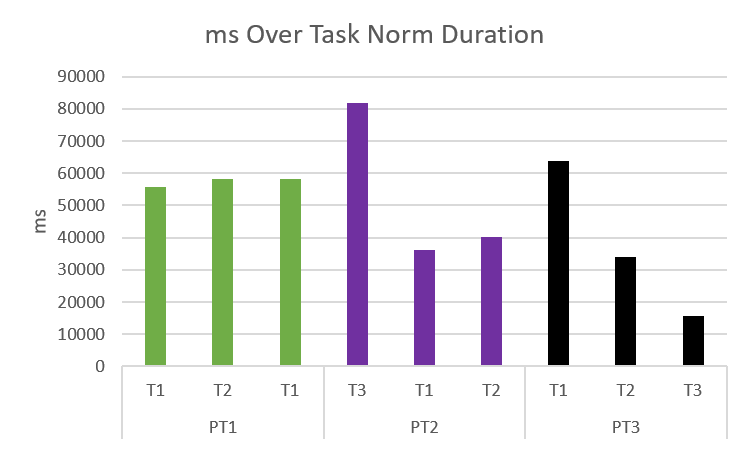
\includegraphics[width=0.8\textwidth]{figures/msOverTaskNorm.png}
	\caption[TCT of all sessions.]{Amount of miliseconds over task norm time (task duration without speed mechanic). PT - participant, T - task.}
	\label{fig:tct}
\end{figure}

\section{Data Analysis}
Based on the pilot study, this section tries to give a first glimpse of the data. The data relies on only three participants. Additionally, the data relies on a pilot study. A pilot study serves to identify issues and faults in the system and study and prepare the final study conduction. Section\todo{55} describes found issues and faults and the solution for them. Some issues and faults impacted the data, which led to the exclusion of corresponding data. Furthermore, as described in section~\ref{sec:studyStructure}, a full counterbalancing of tasks and conditions is possible with nine participants. Additionally, the data revealed, in some aspects, a high variation in both qualitative and quantitative data. Therefore, the depicted data is a rough estimation, and conclusions can not be drawn. The analysis is superficial, and a detailed analysis like significant verification is renounced. However, the first impression of a possible outcome can be given. All charts depicted in this section are similarly structured. The conditions in all charts have the same colour coding: \textcolor{blue}{EGO} is depicted in blue, \textcolor{orange}{EXO} is depicted in orange and the combination \textcolor{gray}{EGO \& EXO} is depicted in gray. For all charts (except for head angle) holds: the lower the bar, the better in the corresponding context.\\
Figure~\ref{fig:cumulatedError} can be perceived as an abstract for this section by showing the overall error in distance and angle between the learner and the GV per VP. Overall, the ego-centric VP mostly outperformed both the exo-centric VP and the ego \& exo-centric VP, while the ego \& exo-centric VP mostly scored better than the exo-centric VP.
\begin{figure}[htb]
	\centering
	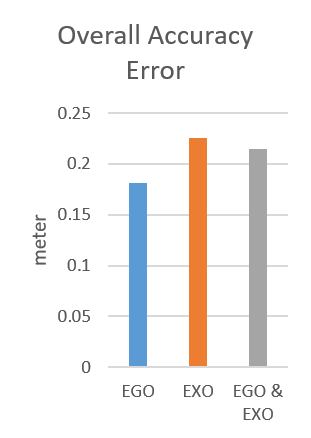
\includegraphics[width=0.3\textwidth]{figures/cumulatedDistanceError.png}
	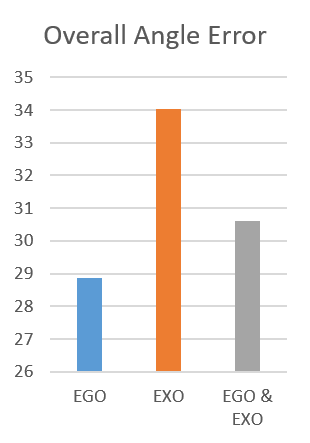
\includegraphics[width=0.3\textwidth]{figures/cumulatedAngleError.png}
	\caption[Cumulated error per perspective.]{Cumulated average distance error (left) and angle error (right) per VP.}
	\label{fig:cumulatedError}
\end{figure}


\subsection{Accuracy}
Accuracy is clustered by distance and angle and applied for the body parts hands, feet, hip, head and box. Distance is the Euclidean distance between the learners, e.g. hand and the GV hand in meters, and describes the difference in position. Angle describes the difference in orientation and is measured in degrees. The overall error per body is depicted in~\ref{fig:overallError}.
Section~\ref{sec:studyStructure} showed that some sub-tasks could be paired up, based on the similarity of the movements: \textit{lift}/\textit{lower}, \textit{push}/\textit{pull}, \textit{turn}/\textit{fold} and \textit{pick}/\textit{place}. Figure~\ref{fig:avgErrorPerSubTask} shows the average error in distance and angle per sub-task and confirms the pairing of the sub-tasks by showing a relation between the pairs. Hence, in the following, the pairs of sub-tasks will be analysed in combination. \textit{Carry} and \textit{walk} are analysed seperately. The sub-tasks structure this section. The sub-task is analysed based on the accuracy measurements and compared with the subjective accuracy of the learner.
\begin{figure}[H]
	\centering
	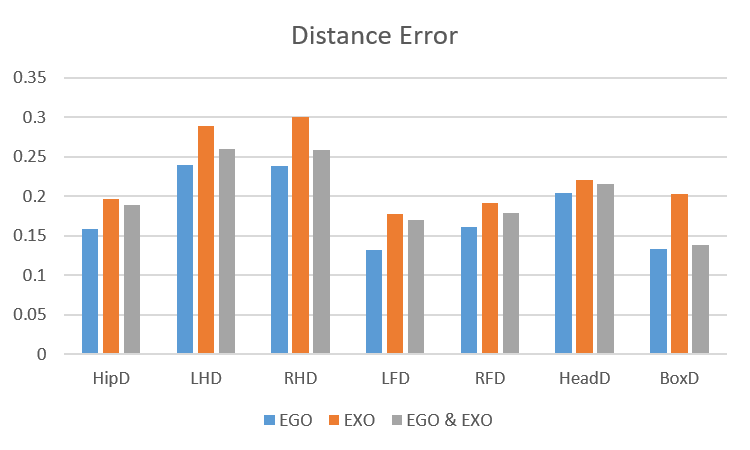
\includegraphics[width=0.49\textwidth]{figures/overallDistanceError.png}
	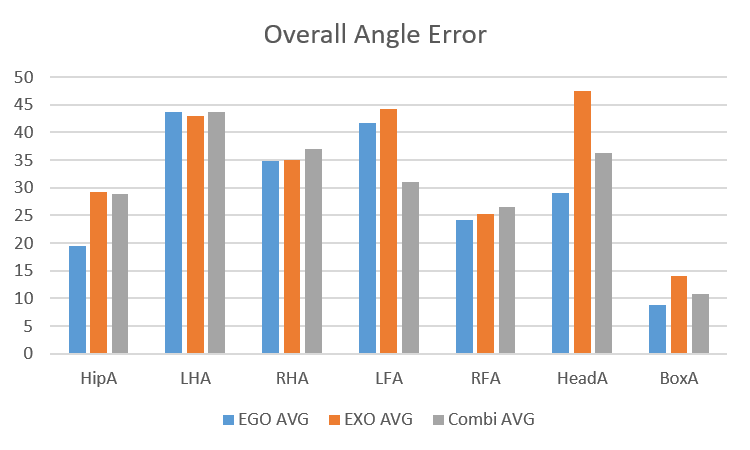
\includegraphics[width=0.49\textwidth]{figures/overallAngleError.png}
	\caption[Average error per body part in meter.]{Average error per body part. Left: distance error, right: angle error. Suffix D: distance, suffix A: angle. LH - left hand, RH - right hand, LF - left foot, RF - right foot.}
	\label{fig:overallError}
\end{figure}
\begin{figure}[H]
	\centering
	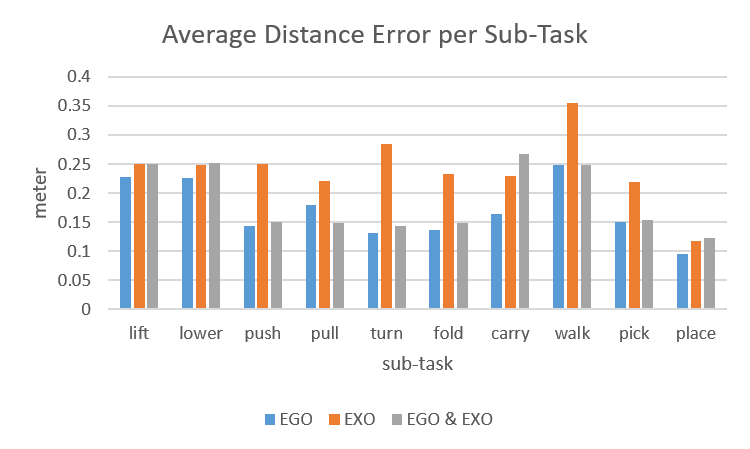
\includegraphics[width=0.49\textwidth]{figures/averageDistanceErrorPerSubTask.png}
	\includegraphics[width=0.49\textwidth]{figures/averageAngleErrorPerSubTask.png}
	\caption[Average error of sub-task\textit{carry}]{Average error of sub-task \textit{carry}. Left: distance error, right: angle error. Suffix D: distance, suffix A: angle. LH - left hand, RH - right hand, LF - left foot, RF - right foot.}
	\label{fig:avgErrorPerSubTask}
\end{figure}

Figure~\ref{fig:overallError} shows that the distance error of hands and the error of feet are related. This is expected since large parts have synchronised movements. For example, the hands touch the box simultaneously. Across all conditions, the feet's error is lower than the hands' error. The hands' error is lower in EGO than in EXO. Hands are directly visible in front of the learner and the direct comparison to the ego-centric GV is a possible explanation. Surprisingly, feet's error is lower in EGO, too. To see the feet, the learner must actively move the head, primarily if the box blocks the view on the feet. However, it seems easier to align the learner's feet with the GV feet in EGO. The box distance and angle error are lower in EGO and \combi. The presence of an ego-centric GV box increases the distance and angle accuracy for the box presumably significantly. The hip error indicates to what extend the learner could determine the correct location. The data indicates that the determination of one's own position and rotation is more straightforward with an ego-centric GV. The head angle is not comparable with the other accuracy measures. The presence of multiple exo-centric GVs in the EXO forces the learner to look into different directions. The difference between EXO and \combi\ could point out that the learner focussed in \combi\ on both the exo-centric GVs and ego-centric GV. The angle-based accuracy for the hand and feet reveal no clear trend. More participants are needed to get a clearer view. Overall, the presence of an ego-centric GV increases the distance accuracy for all body parts. For the box-shaped physical load, the presence of an ego-centric GV increases the angle accuracy, too. On the one hand, adding exo-centric GVs to the ego-centric GV decreases the distance accuracy. A possible reason could be that the learner shares the focus with multiple GVs or that the presence of four exo-centric GVs overwhelms the learner. The study participants rated their overall accuracy highest in EGO and lowest in \combi, compare~\ref{fig:overallSubjectiveAccuracy} (left). The low subjective accuracy in \combi\ would underpin the theory that the learners were overwhelmed. However, when the participants were asked about their subjective accuracy for the body parts, arms, legs and back, a different picture arises, compare~\ref{fig:overallSubjectiveAccuracy} (left). The participants' opinion is differentiated, which causes a high standard deviation of around 1.5 on a Likert scale from 1-7. More participants could lead to a clearer view. On the other hand, adding an ego-centric GV to exo-centric GVs increases the accuracy slightly.\\
The described insights rely on the whole task containing all sub-tasks. The drawn deductions are only valid for a task that includes all sub-tasks in the same amount. Potentially, the accuracy in specific sub-tasks could differ from the overall accuracy. In the following, the sub-tasks are analysed and vetted if the deductions count for the specific sub-tasks.
\begin{figure}[H]
	\centering
	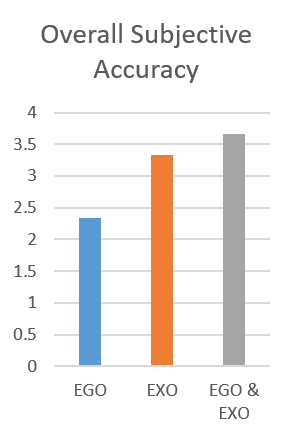
\includegraphics[width=0.3\textwidth]{figures/overallSubjectiveAccuracy.png}\\ 
	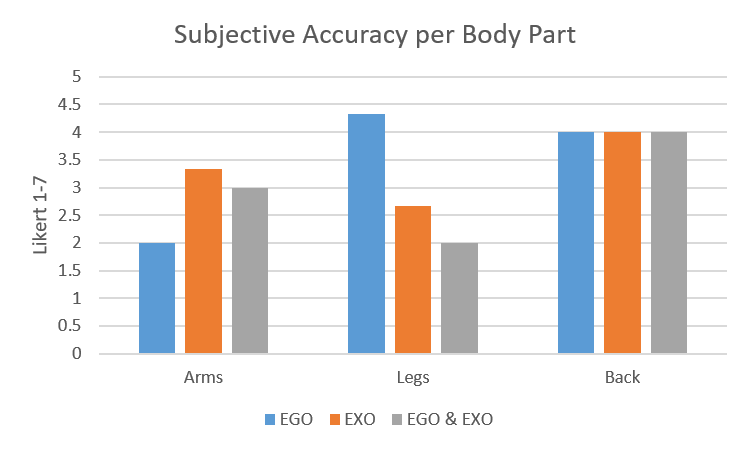
\includegraphics[width=0.49\textwidth]{figures/subjectiveAccuracyPerBodyPart.png}
	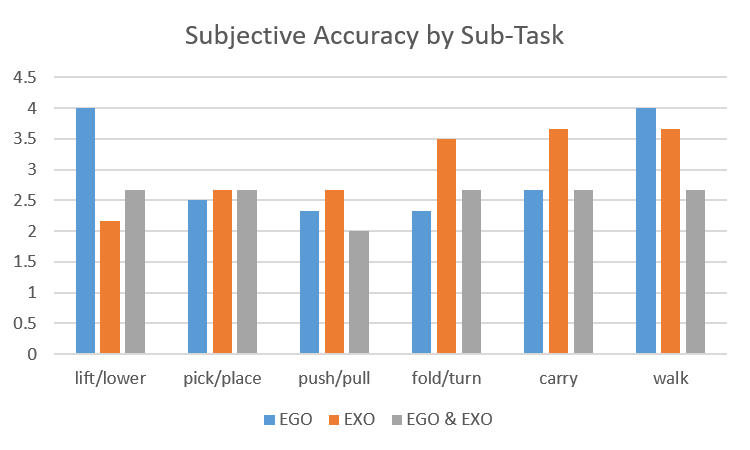
\includegraphics[width=0.49\textwidth]{figures/subjectiveAccuracyBySubTask.png}
	\caption[Subjective accuracy per VP]{Subjective accuracy per VP}
	\label{fig:overallSubjectiveAccuracy}
\end{figure}

\begin{figure}[H]
	\centering
	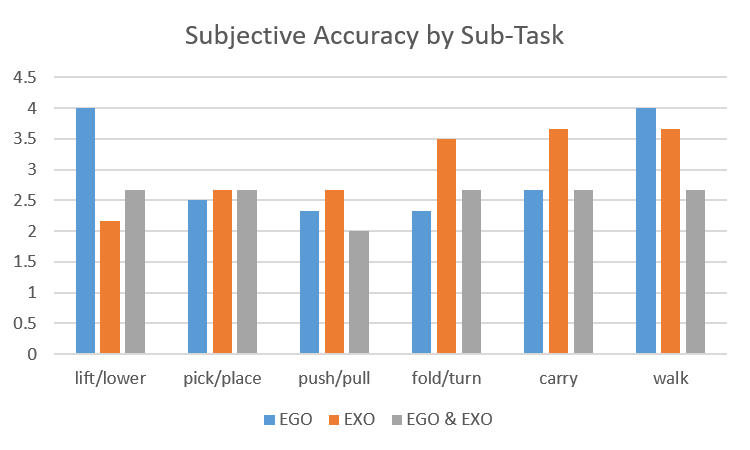
\includegraphics[width=0.29\textwidth]{figures/subjectiveAccuracyBySubTask.png}
	\caption[Subjective accuracy per sub-task]{Subjective accuracy per sub-task}
	\label{fig:subjectiveAccuracybySubTask}
\end{figure}

\subsection{lift/lower}
\begin{figure}[H]
	\centering
	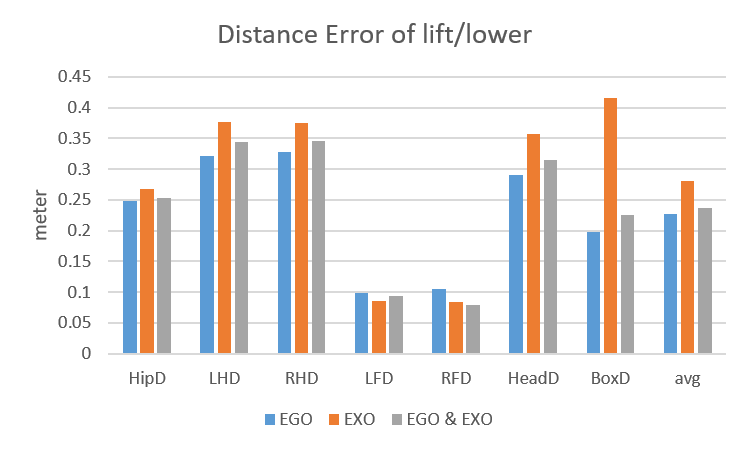
\includegraphics[width=0.49\textwidth]{figures/distanceErrorLiftLower.png}
	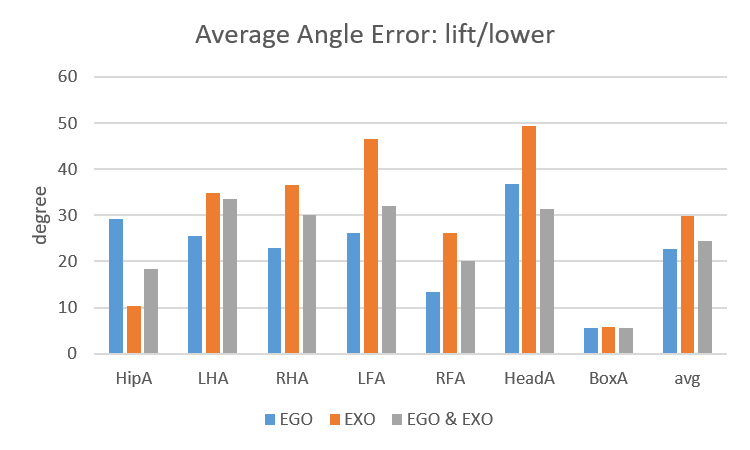
\includegraphics[width=0.49\textwidth]{figures/angleErrorLiftLower.png}
	\caption[Average error per body part for sub-tasks \textit{lift}/\textit{lower}.]{Average error per body part for sub-tasks \textit{lift}/\textit{lower}. Left: distance error, right: angle error. Suffix D: distance, suffix A: angle. LH - left hand, RH - right hand, LF - left foot, RF - right foot.}
	\label{fig:errorLiftLower}
\end{figure}
Figure~\ref{fig:errorLiftLower} shows that in EGO, the hip, hand and head accuracy is higher than in an EXO. The presence of exo-centric GV seems to have a positive influence on the feet's accuracy. The box's accuracy in EXO is lower than in EGO and EXO. In the actual study, particular attention should be paid to the box during \textit{lift} and \textit{lower} to identify the cause of why EXO performed badly. In orientation, the box's error is low for all VPs. This is expected since the sub-task does not include a change in orientation.
The subjective accuracy is by far lowest in EGO, followed by EGO and EXO.

\subsection{pick/place}
\begin{figure}[H]
	\centering
	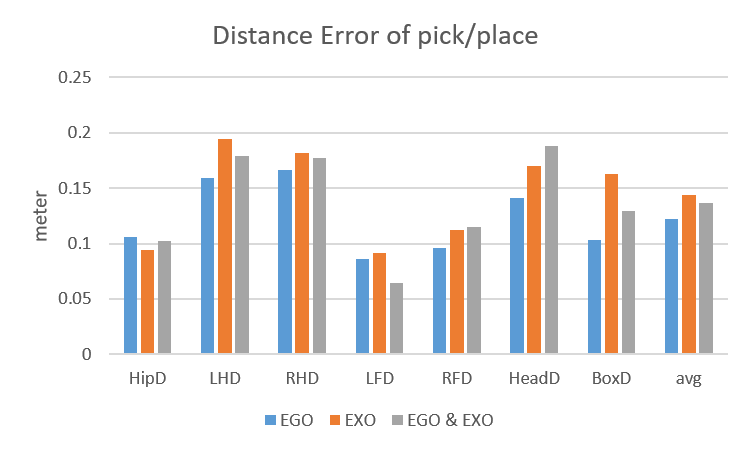
\includegraphics[width=0.49\textwidth]{figures/distanceErrorPickPlace.png}
	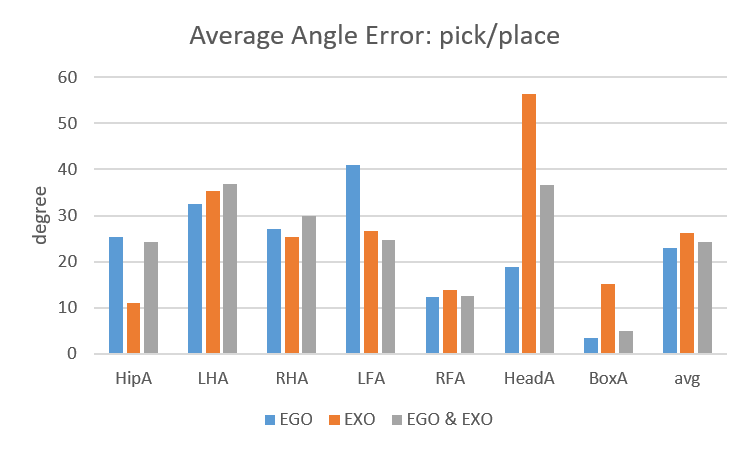
\includegraphics[width=0.49\textwidth]{figures/angleErrorPickPlace.png}
	\caption[Average error per body part for sub-task \textit{turn}/\textit{fold}.]{Average error per body part for sub-task \textit{turn}/\textit{fold}. Left: distance error, right: angle error. Suffix D: distance, suffix A: angle. LH - left hand, RH - right hand, LF - left foot, RF - right foot.}
	\label{fig:errorPickPlace}
\end{figure}
\textit{Pick} and \textit{place} are \textit{lift} and \textit{lower} movements with a significant difference in magnitude. The accuracy of pick and place benefits from the presence of an ego-centric GV. The distance and angle error of the box is lowest in EGO.
\subsection{push/pull}
\begin{figure}[H]
	\centering
	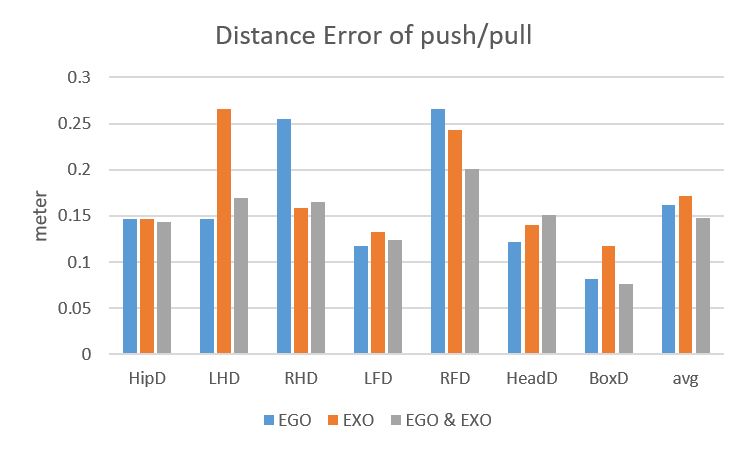
\includegraphics[width=0.49\textwidth]{figures/distanceErrorPushPull.png}
	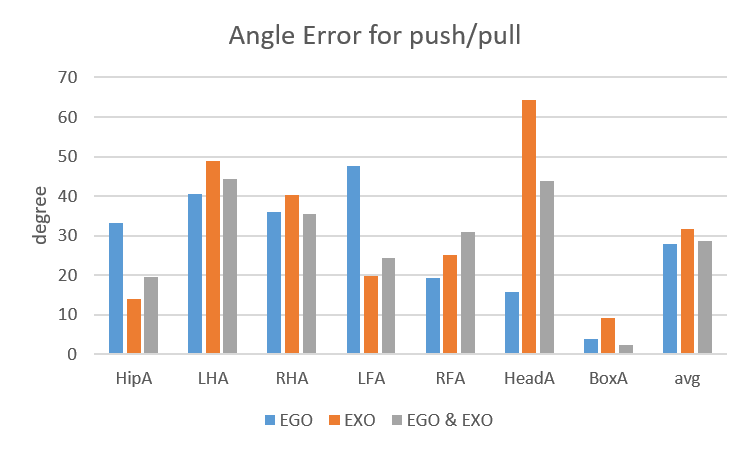
\includegraphics[width=0.49\textwidth]{figures/angleErrorPushPull.png}
	\caption[Average error per body part for sub-tasks \textit{push}/\textit{pull}.]{Average error per body part for sub-tasks \textit{push}/\textit{pull}. Left: distance error, right: angle error. Suffix D: distance, suffix A: angle. LH - left hand, RH - right hand, LF - left foot, RF - right foot.}
	\label{fig:errorPushPull}
\end{figure}
During \textit{push} and \textit{pull}, increased force is applied to the box. The physiologist suggested that one foot should be shifted to the back for \textit{push} and \textit{pull} because of the increased force application. The high difference in error between the left foot and right foot is based on different foot placement. Unfortunately, the participants realised the different foot placement not often. One participant stated that he did not realise to shift one foot back in EGO in the interview. However, in EXO, he saw it and applied it then also for \combi. This statement harmonises with the quantitative data, which shows the lowest accuracy in EGO. The left hand seems to have a high error in EXO, the right hand in EGO. The video revealed that the participants alternated the hand placement during \textit{push} and \textit{pull}. Based on the video observation, the high error could even out with more participants. The higher error of the head angle in EXO compared to \combi\ indicates that the participants shared the focus in \combi\ with the ego-centric GV and the exo-centric GV. The participants rated their movements more exact in \combi\ than in EGO and lowest in EXO.

\subsection{turn/fold}
\begin{figure}[H]
	\centering
	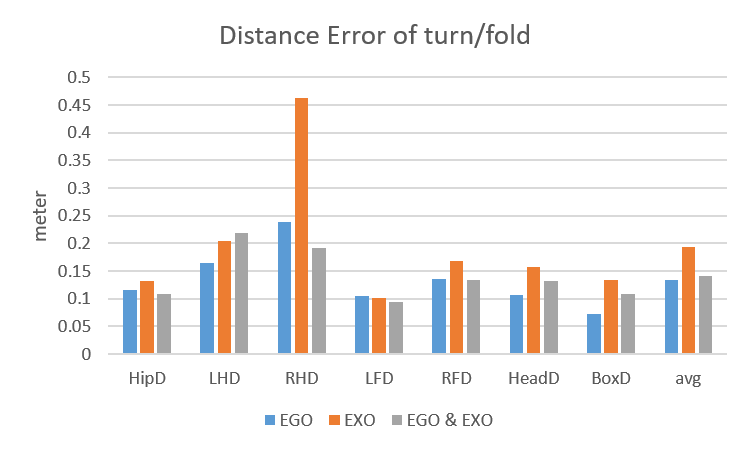
\includegraphics[width=0.49\textwidth]{figures/distanceErrorTurnFold.png}
	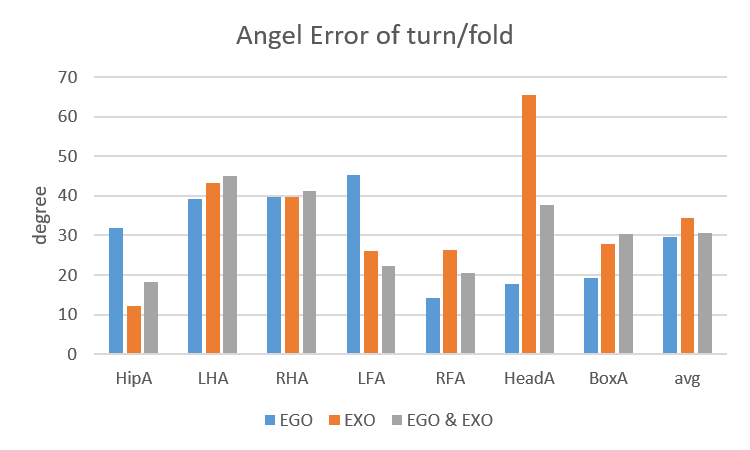
\includegraphics[width=0.49\textwidth]{figures/angleErrorTurnFold.png}
	\caption[Average error per body part for sub-task \textit{turn}/\textit{fold}.]{Average error per body part for sub-task \textit{turn}/\textit{fold}. Left: distance error, right: angle error. Suffix D: distance, suffix A: angle. LH - left hand, RH - right hand, LF - left foot, RF - right foot.}
	\label{fig:errorTurnFold}
\end{figure}
Most of the movements during \textit{turn} and \textit{fold} happened on the table. Thus the main focus is on the hands. The high error in EXO is noticeable. The consultation of the video recordings revealed that in EXO, the participants could not see the direction of \textit{turn} directly and changed the right hand after the movement began. Furthermore, after starting to \textit{turn} or \textit{fold} the box, the participants changed the hand's position, presumably to ease the movement. The perceived accuracy is highest in EGO, followed by \combi\ and EXO. 

\subsection{carry and walk}
\begin{figure}[htb]
	\centering
	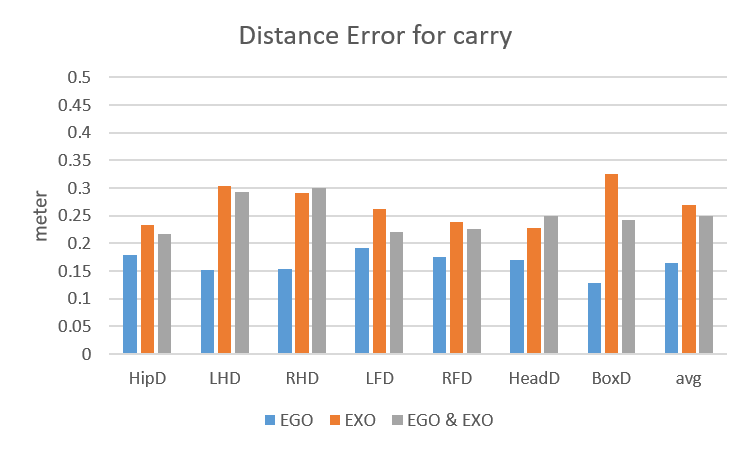
\includegraphics[width=0.49\textwidth]{figures/distanceErrorCarry.png}
	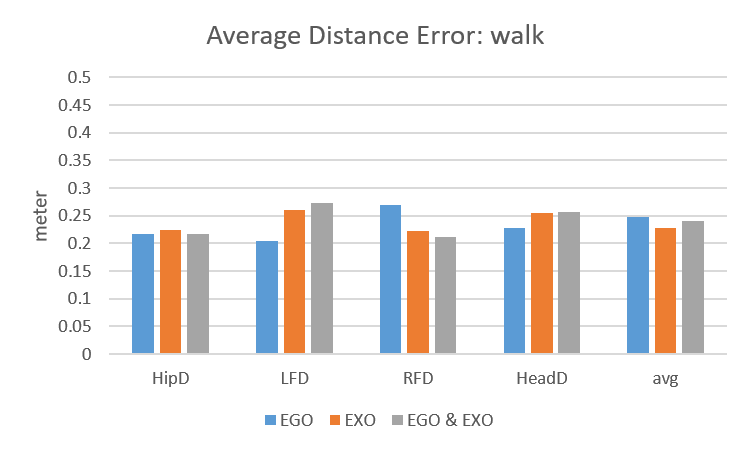
\includegraphics[width=0.49\textwidth]{figures/distanceErrorWalk.png}
	\caption[Average error of sub-tasks \textit{carry} and \textit{walk}]{Average error of sub-tasks  \textit{carry} (left) and \textit{walk} (right). Suffix D: distance. LH - left hand, RH - right hand, LF - left foot, RF - right foot.}
	\label{fig:walkError}
\end{figure}
Teaching locomotion in the ego-centric VP with the help of the \textit{speed mechanic} is a novelty. The data revealed a nearly equal error for ego-centric guided walking and exo-centric guided walking. The position of the hands are not essential for walking and are not depicted. Adding a physical load to walking (\textit{carry}) has a strong influence on accuracy. The learner seems to focus on the box and tries to match the GV's box with the own box. This increases the accuracy of their own position for all body parts.

\section{Visual Focus}
In EGO, the learner is provided one ego-centric GV and will focus on it. If exo-centric GVs are added to the scene, the learner can focus on multiple GVs. Furthermore, it is interesting which percentage of time the learner focuses on the own/GVs box and own/GVs body.\\
\begin{figure}[htb]
	\centering
	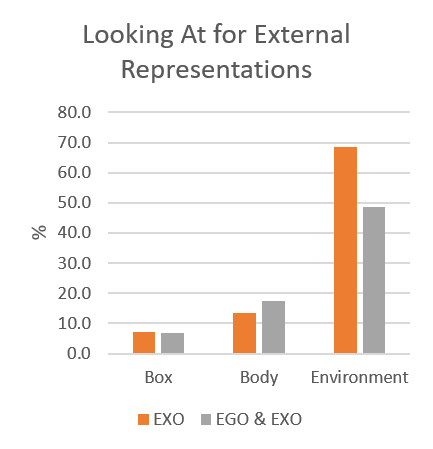
\includegraphics[width=0.5\textwidth]{figures/lookingAtExternalRepresentations.png}
	\caption[Looking At for external representations.]{When looking at an external representation, percentage of time focussing on the box or table.}
	\label{fig:lookingAtExternal}
\end{figure}
A pilot study helps to evaluate the experiment design and data acquisition. Conducting a pilot study before the actual study is vital. The proof is depicted in figure~\ref{fig:lookingAtExternal}. In section~\ref{sec:rayTrace} it is described how the looking at data acquisition method was developed and tested. The formative test was conducted with one person\footnote{More participants were not possible because of the COVID-19 pandemic.}, which is too little. The study data revealed that the data acquisition for looking at is not working correctly. Over 50\% of the time, the ray traces hit the environment. For the actual study, the artefacts and avatars' colliders should be adjusted, or if available, an eye-tracker should be used. Nevertheless, assuming the rays which hit something other than the environment are evenly distributed, some deductions can be made from the acquired data.\\
Figure~\ref{fig:lookingAtExternal} shows the percentage of time the learner focussed on the box, a body (avatar) and the environment. The learner focussed roughly twice as much on a body than on the box.\\
Figure~\ref{fig:posHeatMap} shows the positions of the GVs whereby a GV is the union of body, table and box. The positions are overlayed with a heat map. The orange circles stand for the percentage of time the learner focuses on that position. The heat map provides two insights. First, the presence of an ego-centric GV influences the visual focus of the learner. In EXO, where no ego-centric GV is present, the learner focused 11\% of the time on the own table and box. In \combi, the learner focussed 45\% of the time on the ego-centric GV. If an ego-centric GV is present, it is more frequently focussed than exo-centric GVs. By implication, the learner is consulting the exo-centric GVs, if an ego-centric GV is present.
The second insight regards position four. In EXO and \combi, the learner did not focus on the GV at position four. Position four is superfluous for all three tasks.
\begin{figure}[htb]
	\centering
	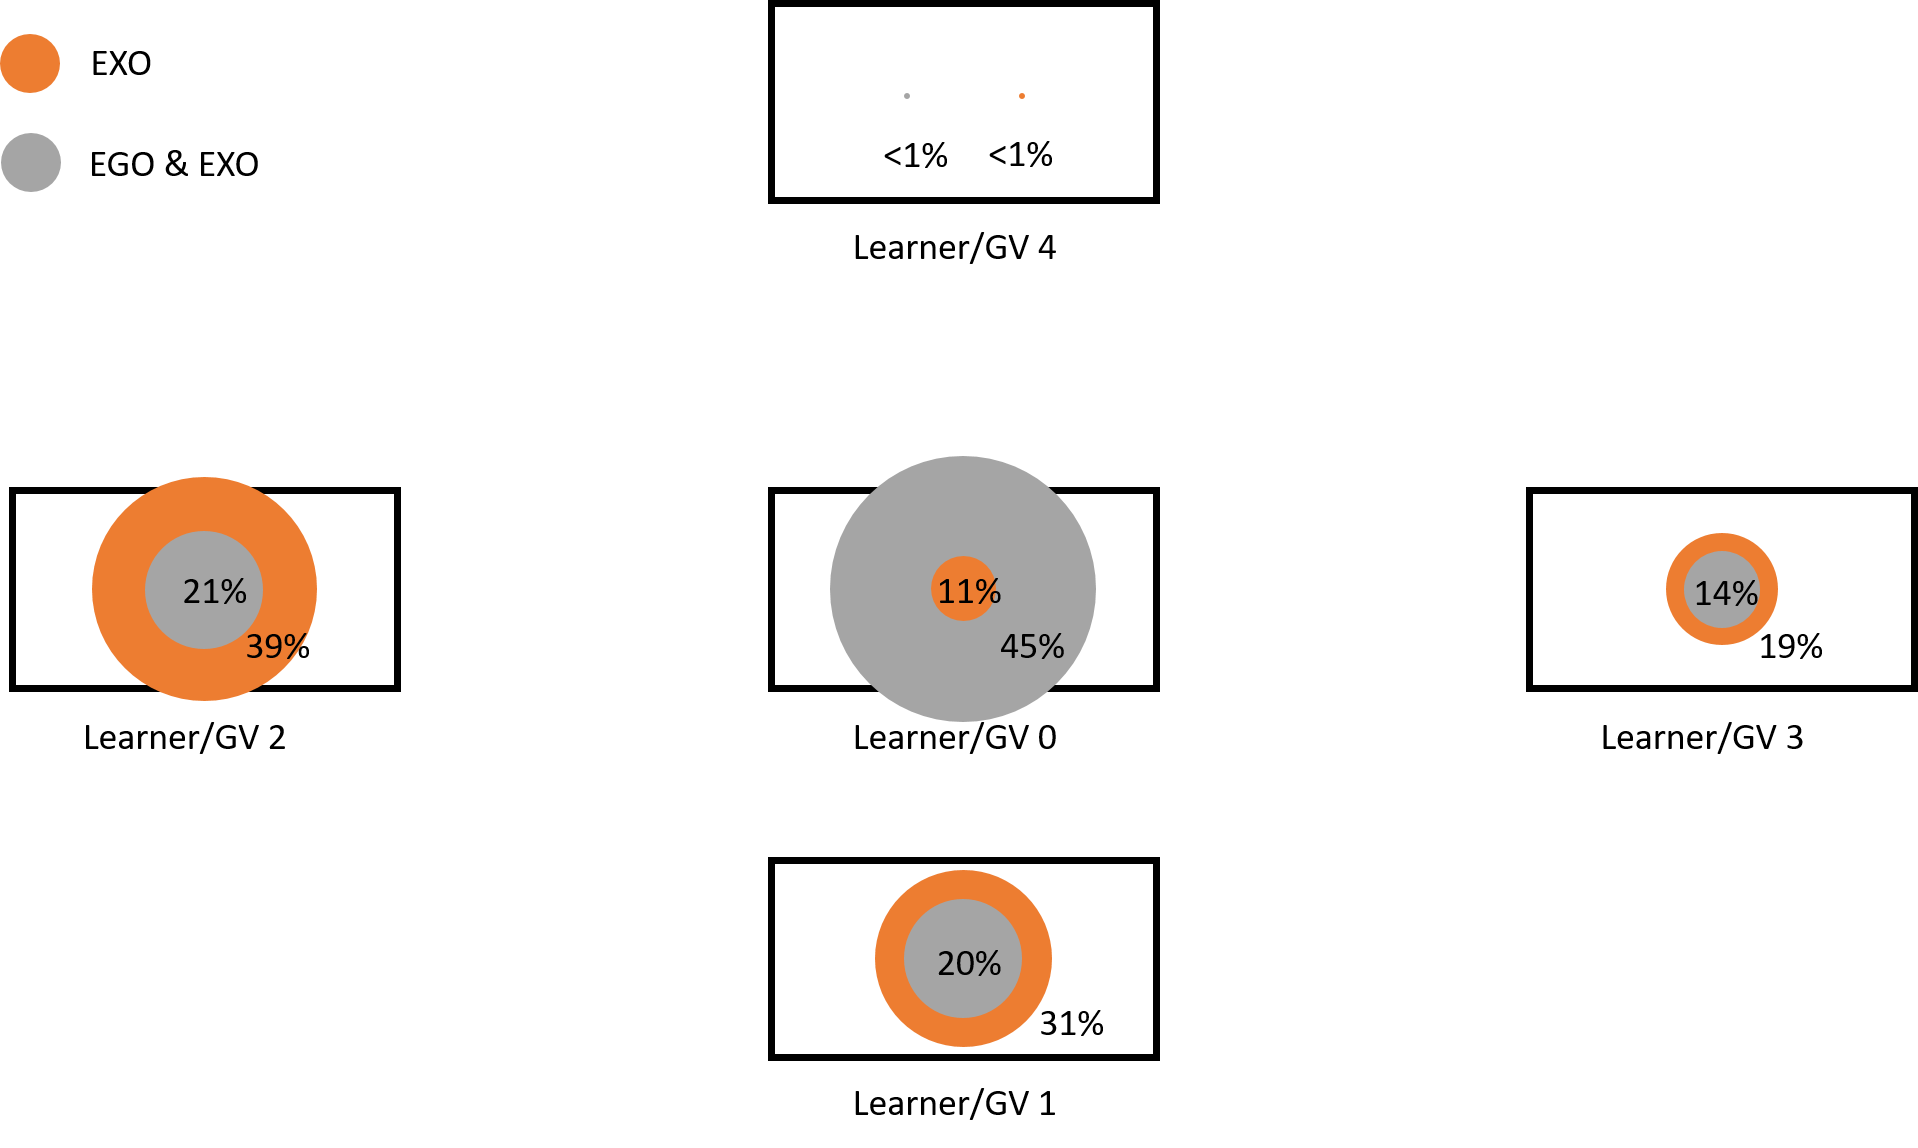
\includegraphics[width=\textwidth]{figures/positionHeatMap.png}
	\caption[\textit{Looking at} heat map.]{Heat map of the learner's focus in EXO and EGO \& EXO. The heatmap shows the tables of the multiple representations. The circles' size corresponds to the amount of time the learner focussed the representation.}
	\label{fig:posHeatMap}
\end{figure}
\todo{perceived acc per body part}

\section{Risk Metrics}
The risk metrics are not analysed. The reason refers to the missing windows the RMs are based on. Recap: for specific sub-tasks the specific RM should be between a minimum and a maximum. The time inside and outside the window between the minimum and maximum yield a score. To determine a window fo the RM a professional should be consulted. Because of the COVID-19 pandemic, a determination by a professional was not possible.\\
However, the accuracy data for \textit{lift} and \textit{lower} could lead to a guess to squat distance performance. The feet accuracy is higher in EXO than in EXO. Squat distance refers to the same body part. Thereby, the assumption seems legit that squat distance could be better in perspectives with an exo-centric GV. Good Base and Spine Bend are referring to body parts that are not directly visible in EGO, though the assumption could be extended to Good Base and Spine Bend, too.

\section{Subjective Preferences}
The personal preferences of the participants tend towards perspectives with exo-centric GVs. If the participants had chosen a VP for the task, two participants would decide for \combi, and one would use EXO. Additionally, two participants stated that they could follow the GV best in \combi, one could follow the GV best in EGO. All but one participant ranked the ability to follow the GV worst in EGO. This competes with the accuracy, which is the lowest in EGO. Surprisingly, all participants stated that the most accessible VP was EGO. In EGO, the GV stands inside the own body, which is not possible in real-world scenarios. Limitation for the ease of understanding is the high proficiency and knowledge about VR of all participants.
